\chapter{Phantom Images}
\label{IEEE}
% New Linearity and PERA software 
% Image comparison (Single, Dual, NEw software) 


\section{Introduction}
In this chapter we outline the reconstruction of the phantom data acquired during our experiments at \acrshort{HSR}. The calibration and event reconstruction was carried out using the BULMA software as the software discussed in chapter \ref{Linearity} was yet to be completed. The series of phantoms shown in this chapter demonstrate the capabilities of the stand alone \acrshort{SPECT} system and the procedures we can carry out to improve the quality of the images. 


\section{Image Reconstruction}
In order to successfully reconstruct the phantom data, all calibration corrections must be applied. Linearity and uniformity maps are applied directly to the planar data, whereas the geometric and sensitivity parameters are applied during reconstruction. The data are reconstructed using Maximum Likelihood Estimation Maximisation (ML-EM), \cite{4307558} in combination with angular blurring, \cite{bousse2013angular},\cite{8069508}. The system calibration determines how the event data are a product of collimator geometry.

\subsection{System Resolution}
The first set of phantoms we consider are the capillary acquired during geometric calibration. Figure \ref{fig_ImageRes} shows capillary phantom reconstructed and combined to give an image of all 60 sources. The image shows promising results across the \acrshort{FOV} as each capillary can be distinguished. We determined the system resolution by modelling the capillary images. The trans-axial resolution was determined at various radial positions across the detector's 20x20x9 $cm^3$ \acrshort{FOV}. A Gaussian model gave the radial and tangential resolution of each trans-axial capillary by the models \acrshort{FWHM}. There was a clear variation with respect to position within the \acrshort{FOV}.

\subsection{Dual Reconstruction}
The reconstruction is limited by the angular sampling of the partial ring collimator. The introduction of a dual reconstruction of two sets of acquisition data allowed us to improve sampling angles. An optional protocol is included; the phantom data may be acquired at two angular positions, separated by a rigid rotation about the z-axis. The second acquisition will provide projections from the missing region of the detector ring; an offset of half a detector also provides data in between each unit and provides improved angular sampling. 

The increase sampling overcomes detection failure over a large area; if a large region is missing, the rotated position is able to capture events from another detector unit. This improves sampling in the system as well as providing a correction for detector failure. The known positions of each acquisition are treated as two subsets, reconstructing both sets of data simultaneously, analogous to an \acrlong{OSEM} (\acrshort{OSEM}) algorithm, \cite{363108}. Each subsequent phantom was reconstructed with this dual method.

\subsection{Partial Volume correction} 
The images were further improved with the introduction of structural information. A simulated \acrshort{MR} acquisition from each phantom was used to determine the geometry and structural information. A post reconstruction \acrlong{PVC} (\acrshort{PVC}) was carried out on the dual reconstructed image. The correction made use of the iterative Yang algorithm, \cite{Erlandsson2012AOncology.}.

\section{Results}
  The results of modelling the capillary phantoms are shown in Fig. \ref{fig_resolution}. Measurements of the radial and tangential resolution show the effects of partial ring geometry; the bottom capillaries in Fig. \ref{fig_ImageRes} are in the region with no detectors and so the reconstructed values have a greater error. The system resolution is most stable closer to the centre of the \acrshort{FOV} where the partial ring effects are less prominent. The standard deviation in resolution is greatest on the edge of the FOV where the point sources appear to stretch radially, Table \ref{table_reso}.
  
\begin{figure}[!t]
%\vspace{-0.2cm}
\centering
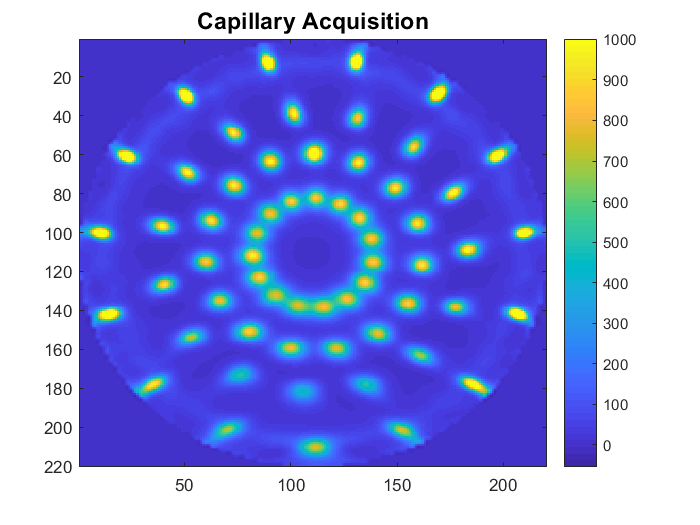
\includegraphics[width=4in]{figures/Capillary_newLRF}

\caption{The reconstructed capillary phantoms after corrections. The capillaries had 1mm diameter; each were filled with 10 MBq of $^{99m}Tc$ and were scanned for 5 minutes.}
\label{fig_ImageRes}
%\vspace{-0.2cm}
\end{figure}

\begin{figure}[!t]
%\vspace{-0.2cm}
\centering
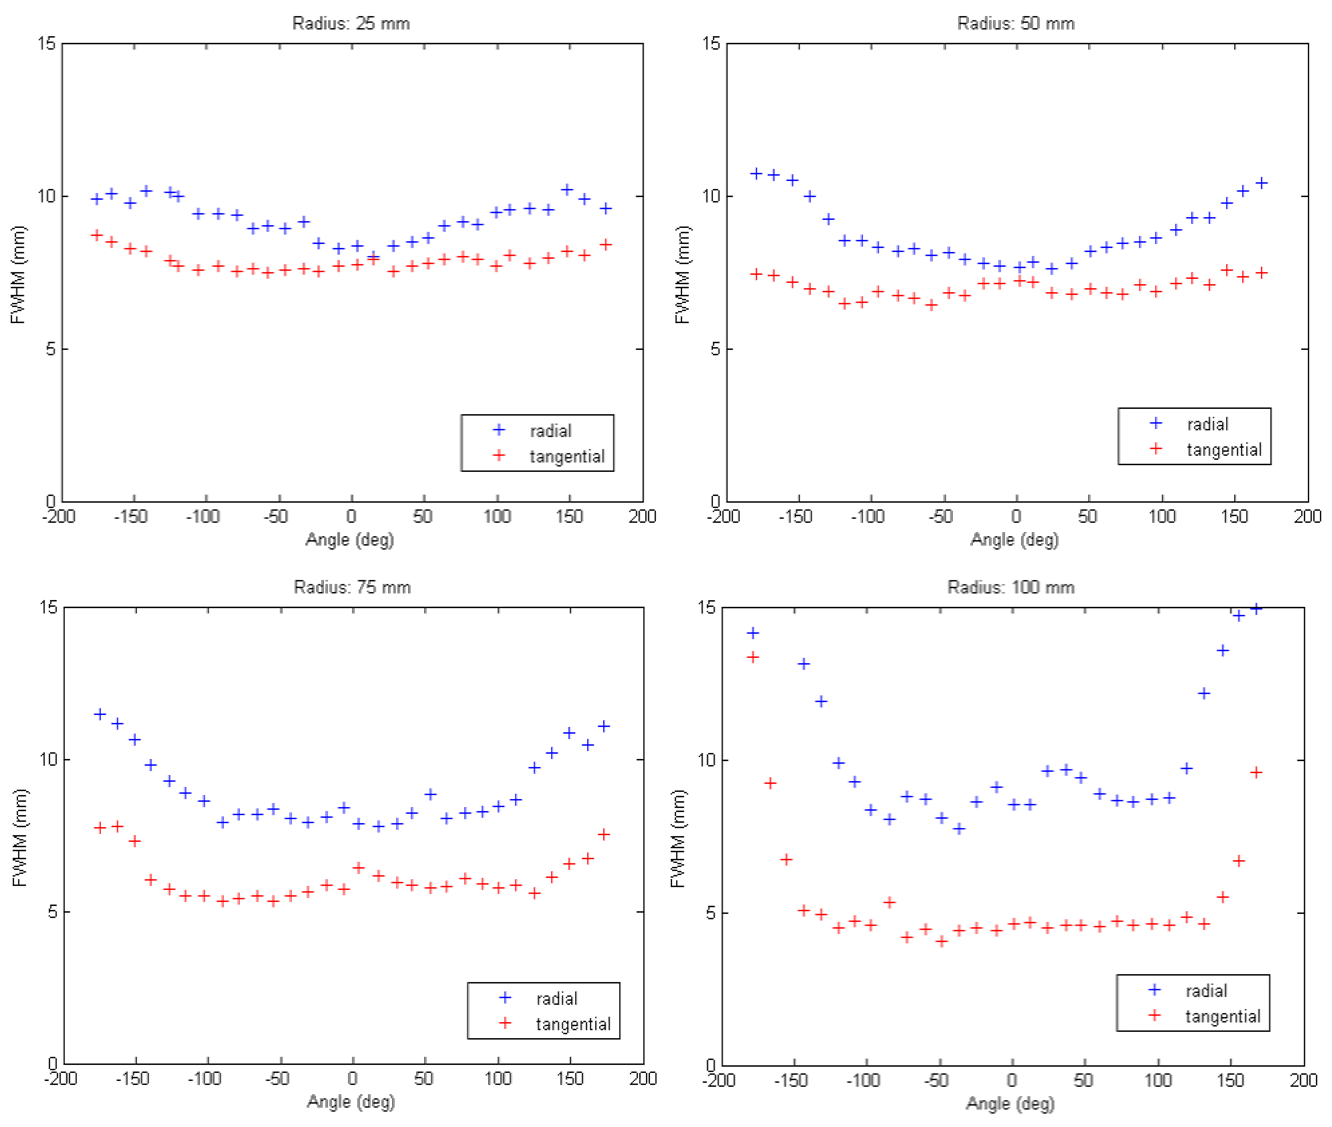
\includegraphics[width=5in]{figures/resolutions.png}

\caption{Resolution of capillaries at 4 radial positions against the angular position in the \acrshort{FOV}}
\label{fig_resolution}
%\vspace{-0.2cm}
\end{figure}

\begin{table}[!b]
% increase table row spacing, adjust to taste
\renewcommand{\arraystretch}{1.3}

\captionsetup{font=small}
\caption{Trans-axial Resolution}
\label{table_reso}
\centering

\begin{tabular}{|p{2.9cm}|p{4.6cm}|p{4.8cm}|}
\hline
Radial Position [mm]& Mean Radial Resolution [mm]& Mean Tangential Resolution [mm] \\
\hline
 25 & 9.39 $\pm$ 0.66 & 7.95 $\pm$ 0.51\\
\hline
 50 & 8.87 $\pm$ 1.15 & 7.31 $\pm$ 0.25\\
\hline
 75 & 9.49 $\pm$ 1.27 & 6.59 $\pm$ 0.95\\
\hline
 100 & 8.83 $\pm$ 2.00 & 5.1629 $\pm$ 1.08\\
\hline
\end{tabular}
\end{table}

 The phantom acquisitions include a Cold Rods phantom, a Hot Spheres phantoms and a 2D Hoffman Brain phantom. Figures, \ref{fig_cold}, \ref{fig_Hot} and \ref{fig_Hoffman}, show the results of the dual reconstruction method and the improvement from the post reconstruction PVC.

\begin{figure}[!t]
%\vspace{-0.2cm}
\centering
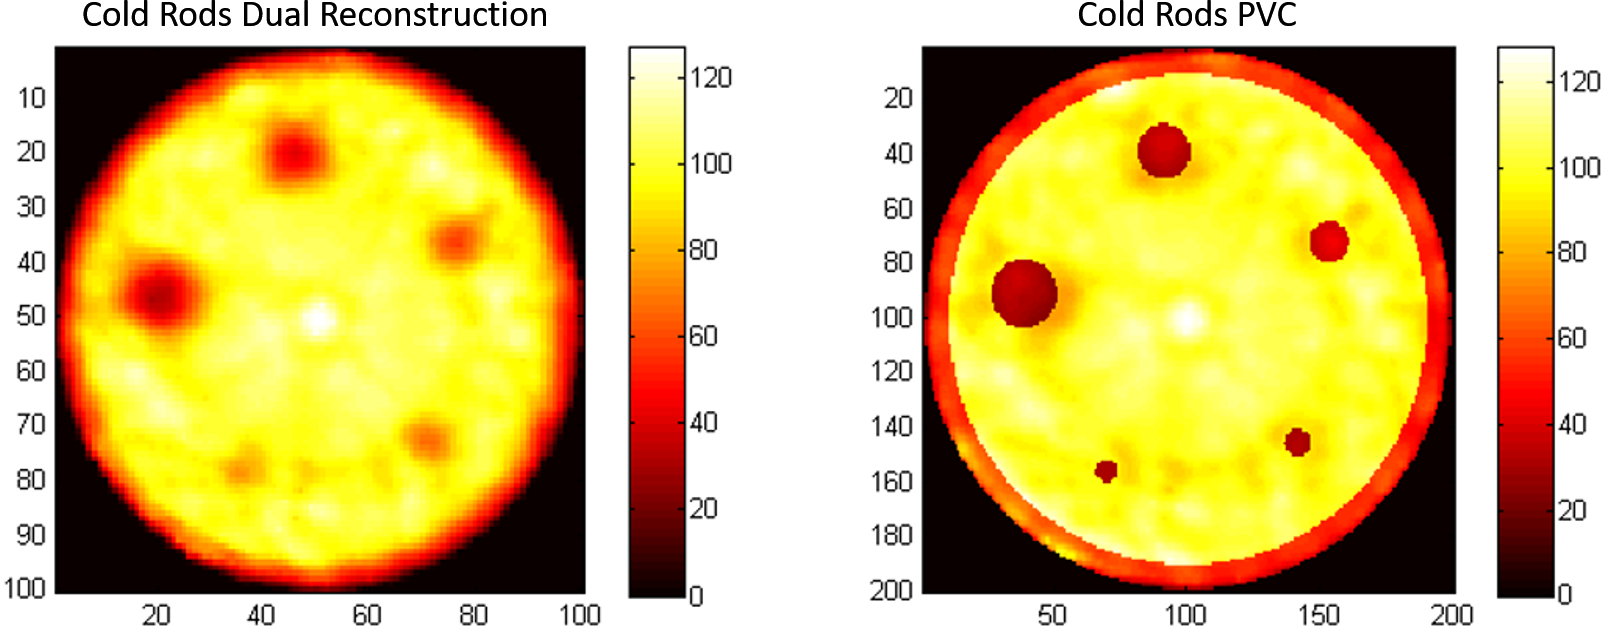
\includegraphics[width=3.5in]{figures/ColdRods.png}

\caption{Cylinder phantom of 50 MBq of activity and cold rods of diameters; 8, 10, 15, 20 and 25 mm.}
\label{fig_cold}
%\vspace{-0.2cm}
\end{figure}

\begin{figure}[!t]
%\vspace{-0.2cm}
\centering
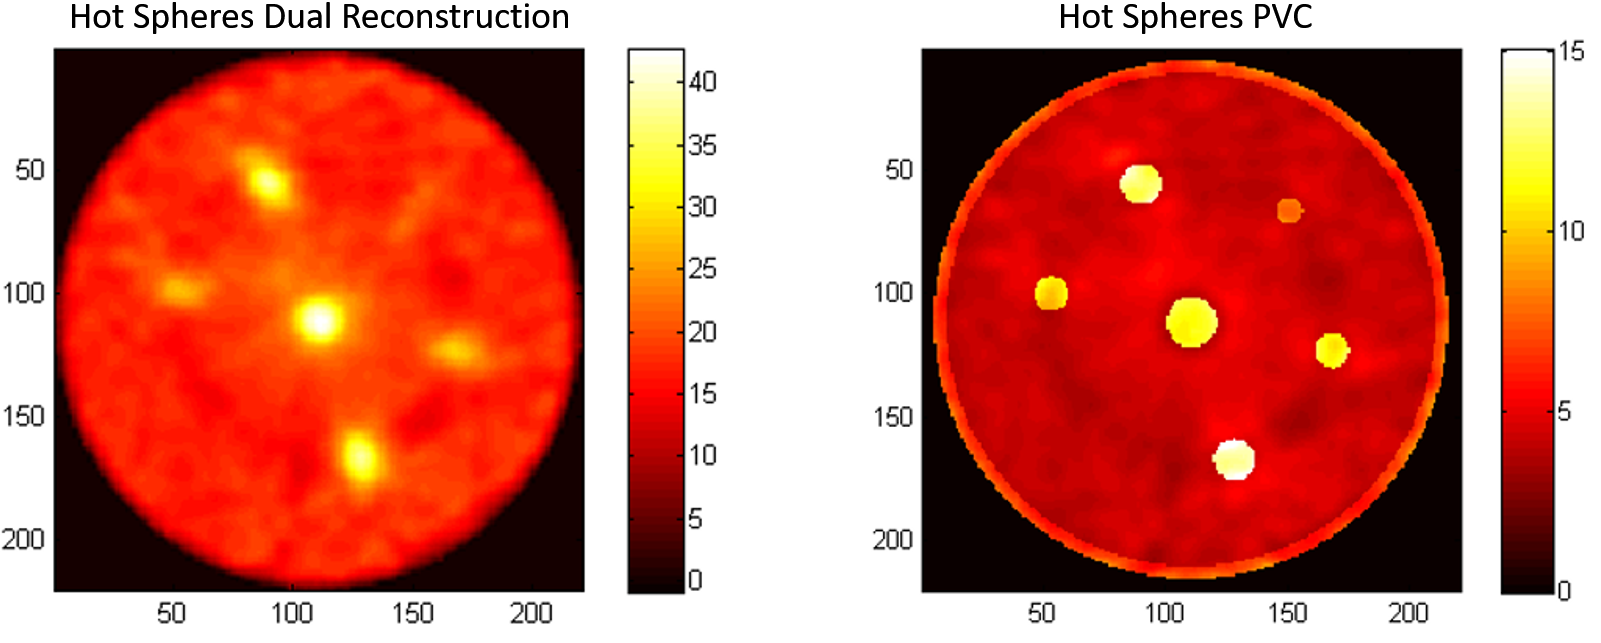
\includegraphics[width=3.5in]{figures/HotSpheres.png}

\caption{60 MBq to a ratio of 8:1 in the hot spheres of diameters; 11, 14, 17, 21 mm.}
\label{fig_Hot}
%\vspace{-0.2cm}
\end{figure}

\begin{figure}[!t]
%\vspace{-0.2cm}
\centering
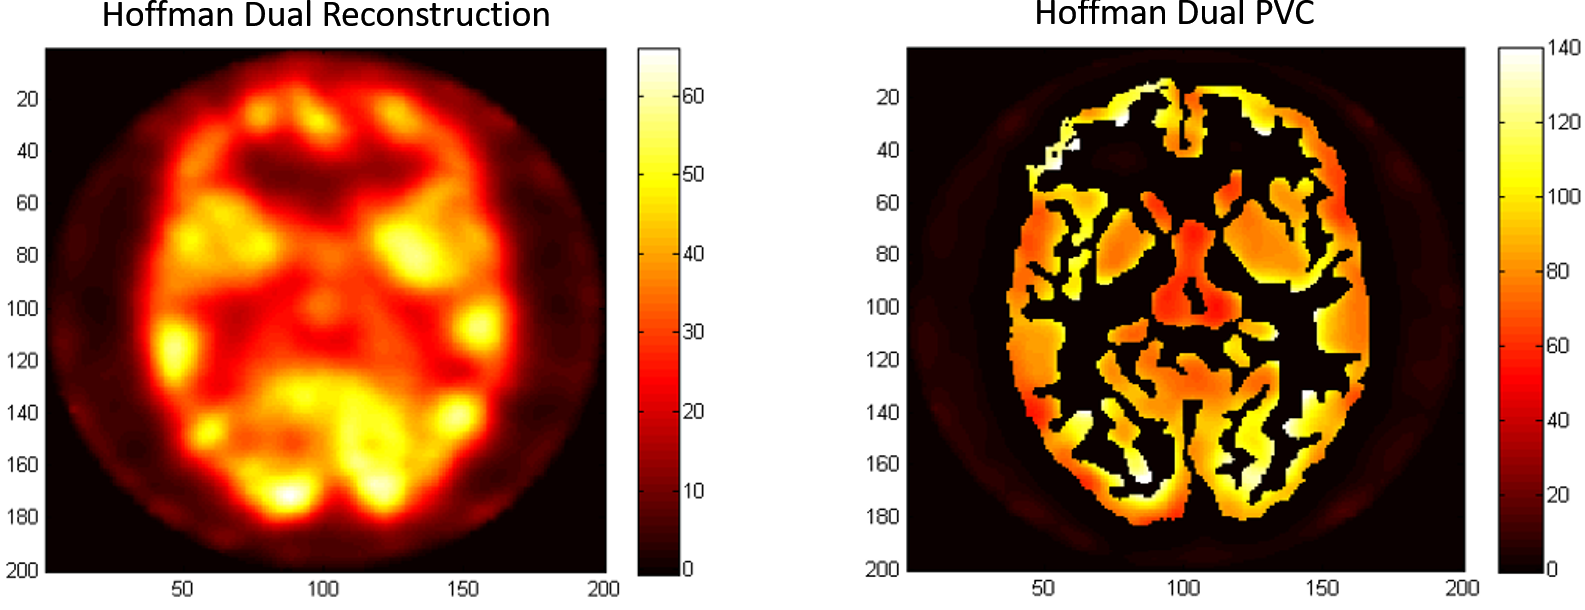
\includegraphics[width=3.6in]{figures/Hoffman.png}

\caption{2D Hoffman phantom with activity 25 MBq.}
\label{fig_Hoffman}
%\vspace{-0.2cm}
\end{figure}

\section{Conclusion}
The results from these phantom reconstruction show promising final images from the desk top \acrshort{SPECT} system. The system shows signs of degradation as the results are worsened compared to previous studies and the intended design specifications. However the age of the detectors are a likely factor in this, \cite{Carminati2019ClinicalCharacterization}. 

We have demonstrated that the performance can be improved with a change of acquisition protocol. Implementing the dual reconstruction has shown to improve the images by improving angular sampling and compensating for faulty acquisitions. However we treat this as an extension to our system, the system is able to function and produce good quality images without this dual acquisition.

The inclusion of \acrshort{PVC} demonstrated the potential of incorporating \acrshort{MRI} data with the \acrshort{SPECT}. However we must reproduce these reconstructions with real \acrshort{MRI} data to verify the results. 

The image quality is strongly related to the stability of the system and the accuracy of the calibration data. It is therefore essential to carry out regular calibration and keep track of the detector stability. Further experiments will set out to improve the image quality and detector stability by incorporating new calibration and acquisition procedures. 

\subsection{Discussion}

Overall the acquisition and reconstruction methods have demonstrated effective means of generating reconstructed images from incomplete data acquisition. We are able to correct for inhomogeneity and pixel failure in the detectors and produce correct projection data. The results of this research improved the processing of \acrshort{INSERT} projection data and introduced dual reconstruction, which can be used to benefit the system's clinical performance. We have determined a set of corrects which can be applied to the BULMA software to aid in the reconstruction of phantom data. 

However it is clear that the instability of the system required further investigation. We are unable to adapt the BULMA software to account for detector failure and new calibration procedures. The implementation a adaptable software will allow us to incorporate further corrects to our data and develop a calibration procedure which can be carried out quickly and effectively. 

The \acrshort{INSERT} has undergone preliminary characterisation of the \acrshort{SPECT} system, however, complete \acrshort{MR} compatibility has only been validated in the preclinical system. Future work will set out to test the system in a clinical \acrshort{MR} environment and to streamline calibration and acquisition procedures for routine use. The use of \acrshort{MR} data will improve the images further and demonstrate the potential of the fully operational system.   

